\documentclass[10pt]{beamer}

\usepackage[utf8]{inputenc}
\usepackage{pgfpages}
\usepackage{dirtree}
\setbeamertemplate{note page}[plain]
\setbeameroption{show notes on second screen =left}
\AtEndNote{\vfill \begin{center} mm:hh \end{center}}
\newcommand{\notedir}[1] {
  \note{\dirtree{#1}}}
\usepackage{tcolorbox}
\usepackage{tikz}
\usepackage{tikz-3dplot}
\usetikzlibrary{intersections,calc,,angles,quotes,through}
\usepackage{amsmath}
\usepackage{graphicx}
\usepackage{cases}
\def \heart {\textcolor{blue}{$\heartsuit$} }
\def \C {\mathcal{C}}
\def \orthog {\underline{\perp}}
\def\arcos{\operatorname{arcos}}
\def \deg {^{\circ}}

\newcommand{\vect}[1] {
  \overrightarrow{#1}}

\tcbset{%
	basic/.style={colframe=black,
		      colback=white,
		      top= 0mm,
		      bottom = 2mm,
		      boxsep=0mm
		      }
}
\tikzset{
    invisible/.style={opacity=0},
    visible on/.style={alt={#1{}{invisible}}},
    alt/.code args={<#1>#2#3}{%
      \alt<#1>{\pgfkeysalso{#2}}{\pgfkeysalso{#3}} % \pgfkeysalso doesn't change the path
    },
  }

    
\begin{document}  
    \beamertemplatenavigationsymbolsempty
    \setlength{\abovedisplayskip}{0pt}
    \setlength{\belowdisplayskip}{0pt}
    \frame{
	  
	  \frametitle{Équations d'éléments 2D.}
	  \begin{columns}[b]
	   \column{.29\textwidth}\centering \underline{Parabole.}
				  \begin{figure}[h]
				  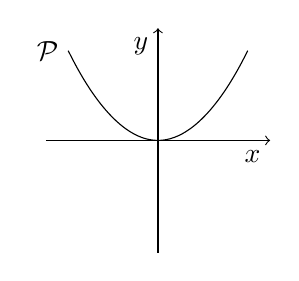
\begin{tikzpicture}[scale=0.57]
					%\draw[help lines] (-3,-3) grid (3,3); 				
					%AXES
					\draw[->] (0,-2.5) -- (0,2.5) coordinate[label=below left:$y$]();
					\draw[->] (-2.5,0) -- (2.5,0) coordinate[label=below left:$x$]();
					
					\draw (-2,2)node[left]{$\mathcal{P}$} parabola bend(0,0) (2,2);
					
				  \end{tikzpicture}
				  \end{figure}
				    $$\mathcal{P} \equiv y = p(x - x_s)^2 + y_s.$$ \smallskip
				    
				  \begin{itemize}
				   \item $(x_s,y_s)$ sommet. \\
				   \item $p$ courbure.
				  \end{itemize}

	   \column{.35\textwidth}\centering\underline{Cercle.}
	   
	   \begin{figure}[h]
				  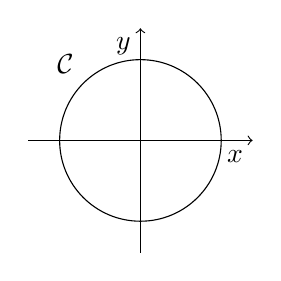
\begin{tikzpicture}[scale=0.57]
					%\draw[help lines] (-3,-3) grid (3,3); 				
					%AXES
					\draw[->] (0,-2.5) -- (0,2.5) coordinate[label=below left:$y$]();
					\draw[->] (-2.5,0) -- (2.5,0) coordinate[label=below left:$x$]();
					
					\draw (0,0) circle (1.8);
					\coordinate[label=above left:$\mathcal{C}$]() at (135:1.8);
					
				  \end{tikzpicture}
				  \end{figure}
				    $$\mathcal{C} \equiv (x-x_s)^2 + (y-y_s)^2 = r^2.$$ \smallskip
				    
				  \begin{itemize}
				   \item $(x_s,y_s)$ centre. \\
				   \item $r$ rayon.
				  \end{itemize}
	   \column{.345\textwidth}\centering\underline{Ellipse.}
	   \begin{figure}[h]
				  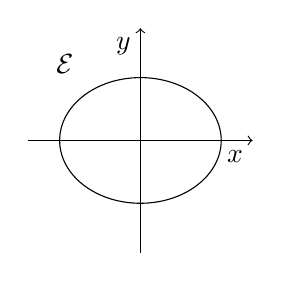
\begin{tikzpicture}[scale=0.57]
					%\draw[help lines] (-3,-3) grid (3,3); 				
					%AXES
					\draw[->] (0,-2.5) -- (0,2.5) coordinate[label=below left:$y$]();
					\draw[->] (-2.5,0) -- (2.5,0) coordinate[label=below left:$x$]();
					
					\draw (0,0) ellipse (1.8cm and 1.4cm);
					\coordinate[label=above left:$\mathcal{E}$]() at (135:1.8);
					
				  \end{tikzpicture}
				  \end{figure}
				    $\mathcal{E} \equiv \frac{(x-x_s)^2}{a^2} + \frac{(y-y_s)^2}{b^2} = 1$. \medskip \vspace{1mm}
				    
				  \begin{itemize}
				   \item $(x_s,y_s)$ centre. \\
				   \item $a,b$ demi-axes.
				  \end{itemize}
	  \end{columns}

	\notedir{%
	.1 Équations d'éléments 2D à connaître.
	.2 Parabole..
	.3 $(x_s,y_s)$ sommet..
	.3 $a$ courbure..
	.4 $a<0$ concavité vers le bas..
	.4 $a>0$ concavité vers le haut..
	.2 Cercle..
	.3 $(x_s,y_s)$ centre..
	.3 $r$ rayon..
	.2 Ellipse..
	.3 $(x_s,y_s)$ centre..
	.3 $a$ demi-axe horizontal..
	.3 $b$ demi-axe vertical..
	}
    }
\frame{\frametitle{Droites perpendiculaires.}
\begin{figure}[h]
				  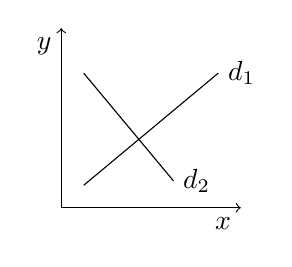
\begin{tikzpicture}[scale=0.57]
					%\draw[help lines] (-3,-3) grid (3,3); 				
					%AXES
					\draw[->] (0,0) -- (0,4) coordinate[label=below left:$y$]();
					\draw[->] (0,0) -- (4,0) coordinate[label=below left:$x$]();
					
					\draw (0.5,0.5) -- (3.5,3)node[right]{$d_1$};
					\draw (0.5,3) -- +(2,-2.4)node[right]{$d_2$};
					
				  \end{tikzpicture}
				  \end{figure}
				  Deux droites sont perpendiculaires $ssi.$ le produit de leur pente vaut -1.
\notedir{%
.1 Droites perpendiculaires.
.2 Droites perp.~ssi produit pente vaut -1..
.3 Explication 'ssi'..
.4 La propriété est vrai dans les 2 sens.
.5 Si deux droites sont perp.~alors le produit vaut -1..
.5 Si le produit vaut -1 alors les deux droites sont perp..
}
}
	  
  
\end{document}

%%% Local Variables:
%%% mode: latex
%%% TeX-master: t
%%% End:
